W świecie gier komputerowych, animacje postaci oraz obiektów odgrywają kluczową rolę w kształtowaniu wrażeń gracza. Optymalne i realistyczne animacje są nieodzowne dla zapewnienia płynnej rozgrywki oraz ułatwienia zanurzenia się w wirtualnym środowisku. W tej sekcji omówione zostaną zaawansowane algorytmy stosowane do animowania postaci, takie jak Blend Trees, Inverse Kinematics (IK) oraz Ragdoll physics oraz animacje interaktywnych obiektów występujące w grze.


\subsubsection{Algorytmy wykorzystywane do animowania postaci}

\textbf{Blend Trees:} Technika Blend Trees jest wykorzystywana w animacjach postaci, umożliwiając płynne przejścia między różnymi animacjami w zależności od czynników takich jak ruch postaci, skok czy interakcje z otoczeniem. W grze jest stosowana dla osiągnięcia bardziej naturalnych i realistycznych animacji postaci.\\
\begin{figure}[h]
    \centering
    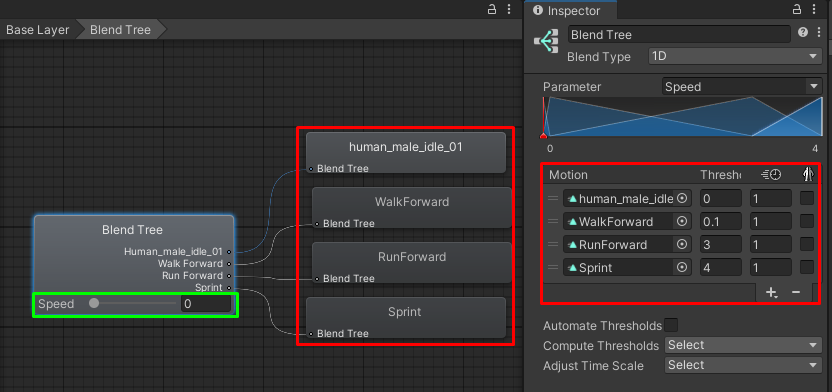
\includegraphics[width=1\linewidth]{Images/blendTree.png}
    \caption{Blend Tree dla płynnego przechodzenia między prędkościami poruszania dla AI}
\end{figure}
\FloatBarrier
\textbf{Inverse Kinematics (IK):}  Algorytm IK to technika matematyczna wykorzystywana w animacji komputerowej do określania pozycji stawów kości w celu osiągnięcia pożądanej pozycji końcowej. W grze IK jest używane do uzyskania bardziej realistycznych ruchów postaci poprzez dynamiczne dostosowywanie rotacji kości. Poniżej znajduje się fragment kodu (\textit{code snippet}), który wykorzystuje IK do dynamicznego dostosowywania rotacji określonych kości postaci przeciwnika, w celu precyzyjnego celowania w kierunku gracza:
\begin{codebox}
\begin{lstlisting}[language={[Sharp]C}, label={listing:WeaponIk.cs}]
public class WeaponIk : MonoBehaviour
{
    // ... (Remaining part of the script)

    private void LateUpdate()
    {
        if (aimTransform == null)
            return;
        if (targetTransform == null)
            return;

        Vector3 targetPosition = GetTargetPosition();

        for(int i = 0; i < iterations; i++)
            for(int j = 0; j < boneTransforms.Length; j++)
            {
                Transform bone = boneTransforms[j];
                float boneWeight = humanBones[j].weight * weight;
                AimAtTarget(bone, targetPosition, boneWeight);
            }
    }

    // ... (Remaining part of the script)
}
\end{lstlisting}
\end{codebox}
\captionof{lstlisting}{Klasa WeaponIk służąca do realistycznego symulowania ruchów kości podczas korzystania z broni przez AI}
\newpage
\textbf{Ragdoll physics:} Algorytm Ragdoll physics symuluje realistyczne reakcje postaci na siły zewnętrzne. W grze jest używany do nadawania postaci dynamicznych właściwości fizycznych po trafieniu lub upadku, co prowadzi do naturalnych animacji. W poniższym fragmencie skryptu odpowiadającym za fizykę ragdoll, zaimplementowano funkcje umożliwiające aktywację i dezaktywację ragdolla, co pozwala na dynamiczną zmianę zachowania postaci w zależności od sytuacji w grze. Dodatkowo, istnieje możliwość zastosowania sił zewnętrznych:
\begin{codebox}
\begin{lstlisting}[language={[Sharp]C}, label={listing:Ragdoll.cs}]
public class Ragdoll : MonoBehaviour
{
    // ... (Remaining part of the script)

    public void ActivateRagdoll()
    {
        foreach (var rigidBody in rigidBodies)
            rigidBody.isKinematic = false;

        if (animator != null)
            animator.enabled = false;
    }
    public void ApplyForce(Vector3 force)
    {
        var rigidBody = animator.
            GetBoneTransform(HumanBodyBones.Hips).
            GetComponent<Rigidbody>();
        rigidBody.AddForce(force, ForceMode.VelocityChange);
    }
}
\end{lstlisting}
\end{codebox}
\captionof{lstlisting}{Skrypt Ragdoll odpowiedzialny za symulowanie realistycznych reakcji postaci na siły zewnętrzne}
\newpage

\subsubsection{Animator przeciwników}
W tej sekcji przedstawiono użycie animatora przeciwników, gdzie wykorzystano warstwę broni wraz z zastosowaniem Avatar Mask. Avatar Mask został użyty do nadpisania animacji dla konkretnych części ciała przeciwnika. W tym przypadku zmienione zostało zachowanie głowy, tułowia oraz rąk podczas odtwarzania animacji na warstwie broni. Celem było zachowanie ruchu nóg z warstwy domyślnej do poruszania się, ale dostosowanie reszty kości do animacji wyciągania/trzymania/chowania broni.
\begin{figure}[h]
    \centering
    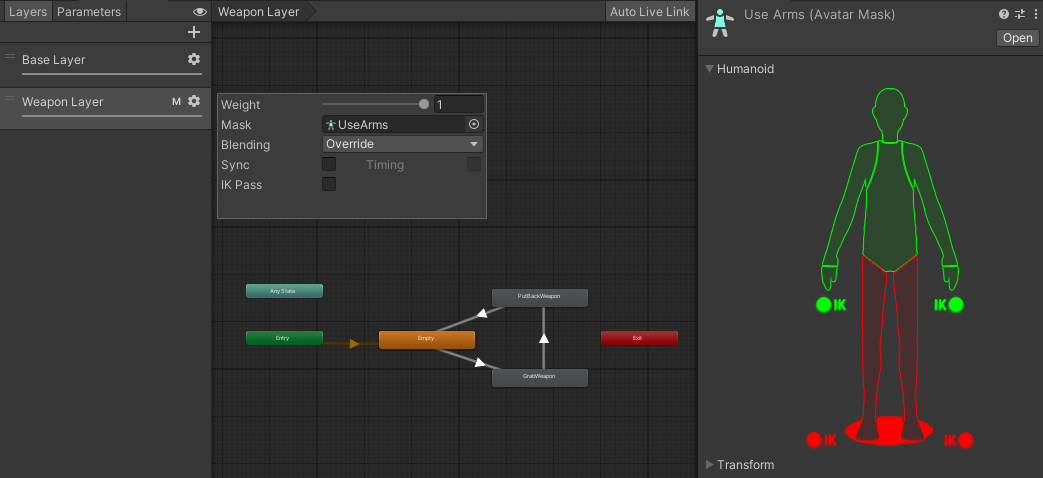
\includegraphics[width=1\linewidth]{Images/aiAnimatorController.png}
    \caption{Warstwa broni Animatora przeciwników i zastosowanie Avatar Maska}
\end{figure}

\subsubsection{Animator otwieralnych/zamykalnych obiektów}
W tej sekcji znajduje się animator otwieralnych i zamykanych obiektów, z ilustracją przykładowej skrzynki. W animatorze umieszczono dwie proste animacje: jedną z otwartą skrzynką, a drugą z zamkniętą. Zastosowano również parametr bool, który jest sterowany z poziomu kodu. Parametr ten działa na zasadzie toggla, co oznacza, że przy zmianie stanu otwiera lub zamyka skrzynkę, co skutkuje odtworzeniem odpowiedniej animacji.
\begin{figure}[h]
    \centering
    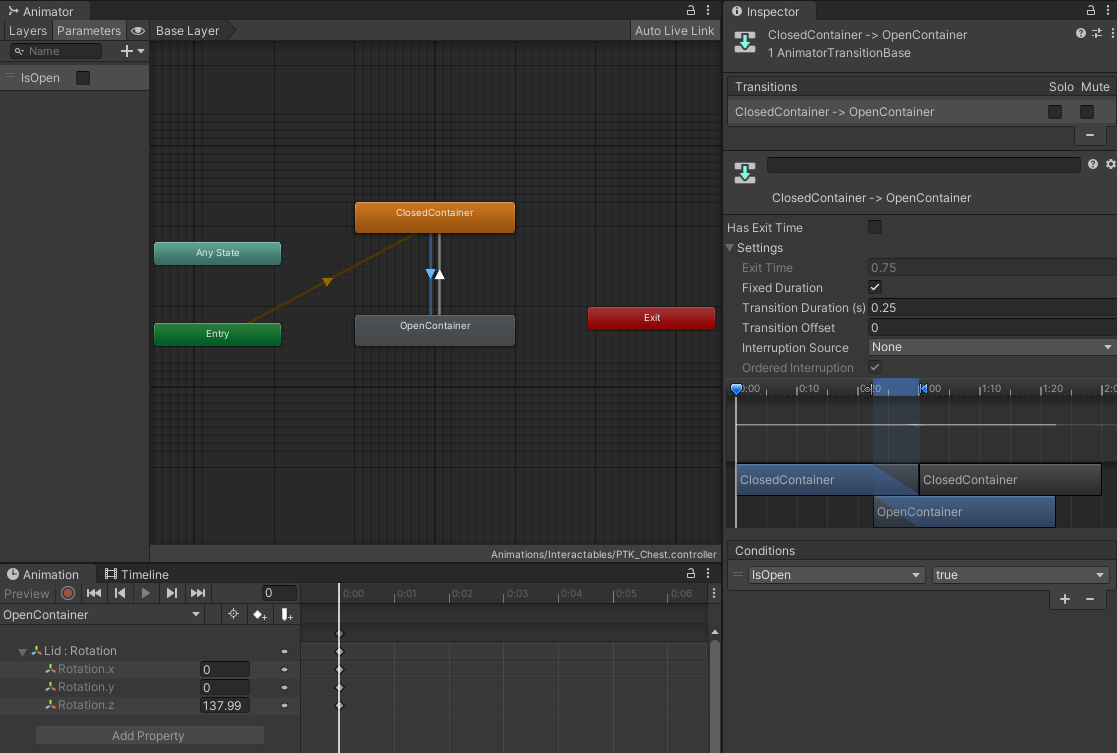
\includegraphics[scale=0.3]{Images/containerAnimator.png}
    \caption{Animator otwieralnego oraz zamykalnego obiektu na przykładzie skrzynki}
\end{figure}
\FloatBarrier